\section{Modelo de grafo en Neo4j}
\label{cap:neo4j}

Neo4j modela las relaciones entre usuarios, canciones y artistas; sobre ese grafo se calculan afinidades, comunidades, recomendaciones y la diversidad de escucha. El código está en \code{databases/neo4j/}, y el análisis de comunidades usa NetworkX.

\subsection{Nodos y relaciones}

La figura~\ref{fig:grafo} muestra el modelo y las tablas~\ref{tab:neo4j-nodos} y~\ref{tab:neo4j-relaciones} detallan las propiedades.

\begin{figure}[H]
\caption{Modelo de grafo}
\label{fig:grafo}
\centering
\begin{tikzpicture}[
  nodo/.style={draw, circle, minimum size=1.7cm, align=center, font=\small},
  rel/.style={-{Stealth[length=2.2mm]}, semithick},
  etiqueta/.style={font=\scriptsize, fill=white, inner sep=1.5pt}]
  \node[nodo] (u) {Usuario};
  \node[nodo, right=3.4cm of u] (c) {Canción};
  \node[nodo, below=2.2cm of c] (a) {Artista};
  \node[nodo, right=3.4cm of a] (com) {Comunidad};
  \node[nodo, below=2.2cm of u] (l) {Lote};
  \node[nodo, below=1.6cm of l] (an) {Análisis};
  \draw[rel] (u) -- node[etiqueta, above] {ESCUCHO} (c);
  \draw[rel] (c) -- node[etiqueta, right] {INTERPRETADA\_POR} (a);
  \draw[rel] (u) -- node[etiqueta, sloped, above] {ESCUCHA\_ARTISTA} (a);
  \draw[rel] (a) -- node[etiqueta, above] {PERTENECE\_A} (com);
  \draw[rel] (a) to[out=-60, in=-120, looseness=5] node[etiqueta, below] {AFIN\_A} (a);
  \draw[rel] (l) -- node[etiqueta, right] {ANALISIS\_ACTIVO} (an);
\end{tikzpicture}
\end{figure}

\begin{table}[H]
\centering
\caption{Nodos del grafo}
\label{tab:neo4j-nodos}
\begin{tabularx}{\textwidth}{l l Y}
\toprule
Etiqueta & Clave única & Otras propiedades \\
\midrule
\code{Usuario} & \code{id} (\code{user_id}) & -- \\
\code{Cancion} & \code{id} (\code{recording_msid}) & \code{titulo} \\
\code{Artista} & \code{nombre} & -- \\
\code{Lote} & \code{id} & \code{source_sha256}, \code{registros}, \code{estado} (cargando o completo) \\
\code{Analisis} & \code{id} & Parámetros, versión de NetworkX, indicadores del análisis y \code{estado} \\
\code{Comunidad} & \code{id} & \code{analisis}, \code{numero}, \code{artistas}, \code{audiencia}, \code{representantes} \\
\bottomrule
\end{tabularx}
\end{table}

\begin{table}[H]
\centering
\caption{Relaciones del grafo}
\label{tab:neo4j-relaciones}
\begin{tabularx}{\textwidth}{l l Y}
\toprule
Relación & Entre & Propiedades \\
\midrule
\code{ESCUCHO} & Usuario $\rightarrow$ Canción & \code{lote}, \code{cantidad}, \code{primera_escucha}, \code{ultima_escucha} \\
\code{INTERPRETADA_POR} & Canción $\rightarrow$ Artista & \code{lote} \\
\code{ESCUCHA_ARTISTA} & Usuario $\rightarrow$ Artista & \code{lote}, \code{cantidad}, \code{proporcion}, \code{primera_escucha}, \code{ultima_escucha} \\
\code{AFIN_A} & Artista -- Artista & \code{analisis}, \code{jaccard}, \code{usuarios_comunes}, audiencias de ambos artistas \\
\code{PERTENECE_A} & Artista $\rightarrow$ Comunidad & \code{analisis}, \code{puente} \\
\code{ANALISIS_ACTIVO} & Lote $\rightarrow$ Análisis & -- \\
\bottomrule
\end{tabularx}
\end{table}

Una relación \code{ESCUCHO} resume todas las reproducciones de un usuario a una canción (cantidad, primera y última fecha); \code{ESCUCHA_ARTISTA} hace lo mismo por artista y añade la proporción que representa en el historial del usuario. Esto reduce las 4,86 millones de escuchas a 1\,791\,408 relaciones \code{ESCUCHO} y 743\,531 \code{ESCUCHA_ARTISTA}. Las canciones se identifican por \code{recording_msid}, cada relación lleva su lote, y las claves únicas se garantizan con restricciones (\texttt{CREATE CONSTRAINT ... REQUIRE n.id IS UNIQUE}).

La figura~\ref{fig:neo4j-browser} muestra el grafo cargado en Neo4j Browser: Linkin Park, el artista con más oyentes (sección~\ref{cap:kpis}), y los 21 artistas con los que tiene una relación \code{AFIN_A}.

\begin{figure}[H]
\caption{Afinidades de Linkin Park en Neo4j Browser}
\label{fig:neo4j-browser}
\centering
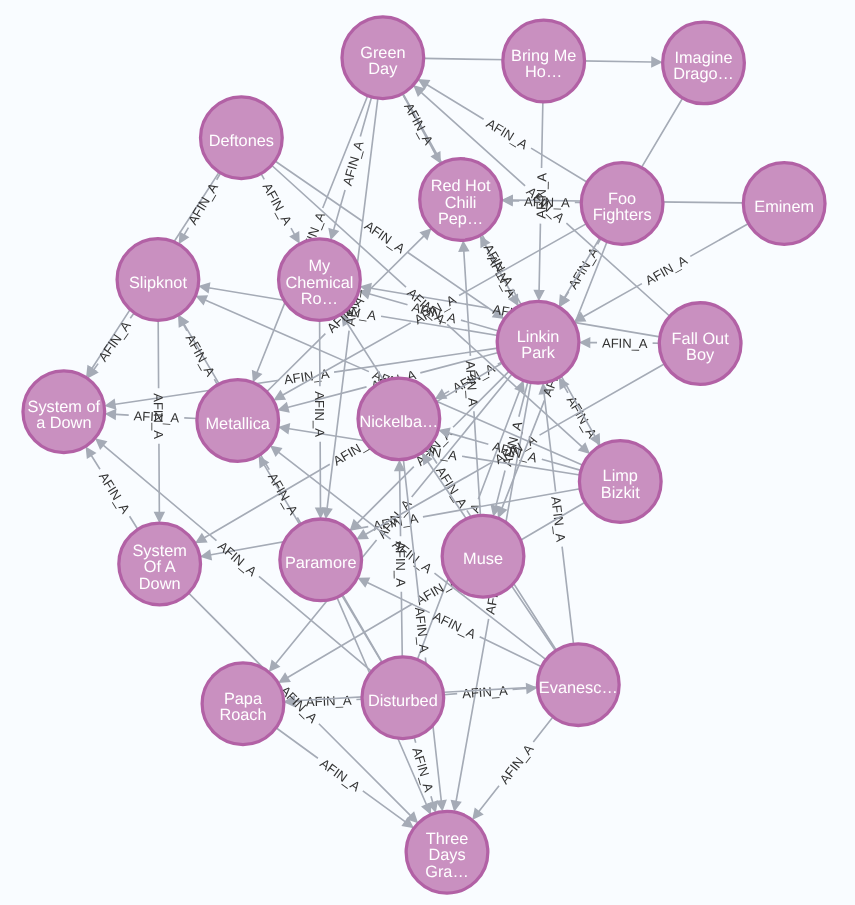
\includegraphics[width=0.62\textwidth]{figuras/neo4j_browser.png}
\end{figure}

\subsection{Carga}

La carga tiene dos etapas. \code{prepare} recorre el JSONL completo, valida cada fila, calcula el SHA-256 del archivo y agrega usuarios, canciones, artistas y pares usuario--canción y usuario--artista en un SQLite intermedio (\code{data/neo4j/prepared.sqlite}). Después \code{load_data} crea las restricciones, registra el nodo \code{Lote} en estado \code{cargando} y envía los datos en lotes de 1000 filas con \texttt{UNWIND} y \texttt{MERGE}, primero nodos y luego relaciones. Al final reconcilia que la cantidad de relaciones y la suma de \code{cantidad} coincidan con lo preparado, y solo entonces el lote pasa a \code{completo}. Como todo usa \texttt{MERGE}, repetir la carga no duplica nada.

\begin{lstlisting}[language=Cypher]
UNWIND $rows AS f
MATCH (u:Usuario {id:f.user}), (c:Cancion {id:f.track})
MERGE (u)-[r:ESCUCHO {lote:$dataset}]->(c)
SET r.cantidad=f.count, r.primera_escucha=f.first, r.ultima_escucha=f.last
\end{lstlisting}

La tabla~\ref{tab:neo4j-carga} resume la carga completa del incremental 2746.

\begin{table}[H]
\centering
\caption{Resultado de la carga completa en Neo4j}
\label{tab:neo4j-carga}
\begin{tabular}{l r}
\toprule
Medida & Resultado \\
\midrule
Escuchas procesadas & 4\,855\,809 \\
Usuarios & 26\,394 \\
Canciones (\code{recording_msid}) & 1\,420\,842 \\
Nombres de artista & 286\,291 \\
Relaciones \code{ESCUCHO} & 1\,791\,408 \\
Relaciones \code{ESCUCHA_ARTISTA} & 743\,531 \\
Relaciones \code{INTERPRETADA_POR} & 1\,424\,734 \\
Preparación en SQLite & 60,20~s \\
Carga en Neo4j & 174,90~s \\
Análisis y publicación & 3,64~s \\
\bottomrule
\end{tabular}
\end{table}

\subsection{Operaciones CRUD en Cypher}

\code{python -m databases.neo4j.crud --pause} trabaja sobre nodos \code{ManagedRecord} para no tocar el lote: crea un usuario y una canción de prueba, los une con \code{ESCUCHO}, actualiza \code{cantidad}, consulta el cambio y elimina relación y nodos con \texttt{DETACH DELETE}.

\begin{lstlisting}[language=Cypher]
MATCH (u:Usuario:ManagedRecord {id:-120012, grupo:$group})
MATCH (c:Cancion:ManagedRecord {id:'manual-track', grupo:$group})
MERGE (u)-[r:ESCUCHO {lote:$group}]->(c)
SET r.cantidad=1
RETURN type(r) AS relacion, r.cantidad AS cantidad
\end{lstlisting}

La figura~\ref{fig:neo4j-crud} muestra la demostración sobre el grafo completo.

\begin{figure}[H]
\caption{Demostración del CRUD en Neo4j}
\label{fig:neo4j-crud}
\centering
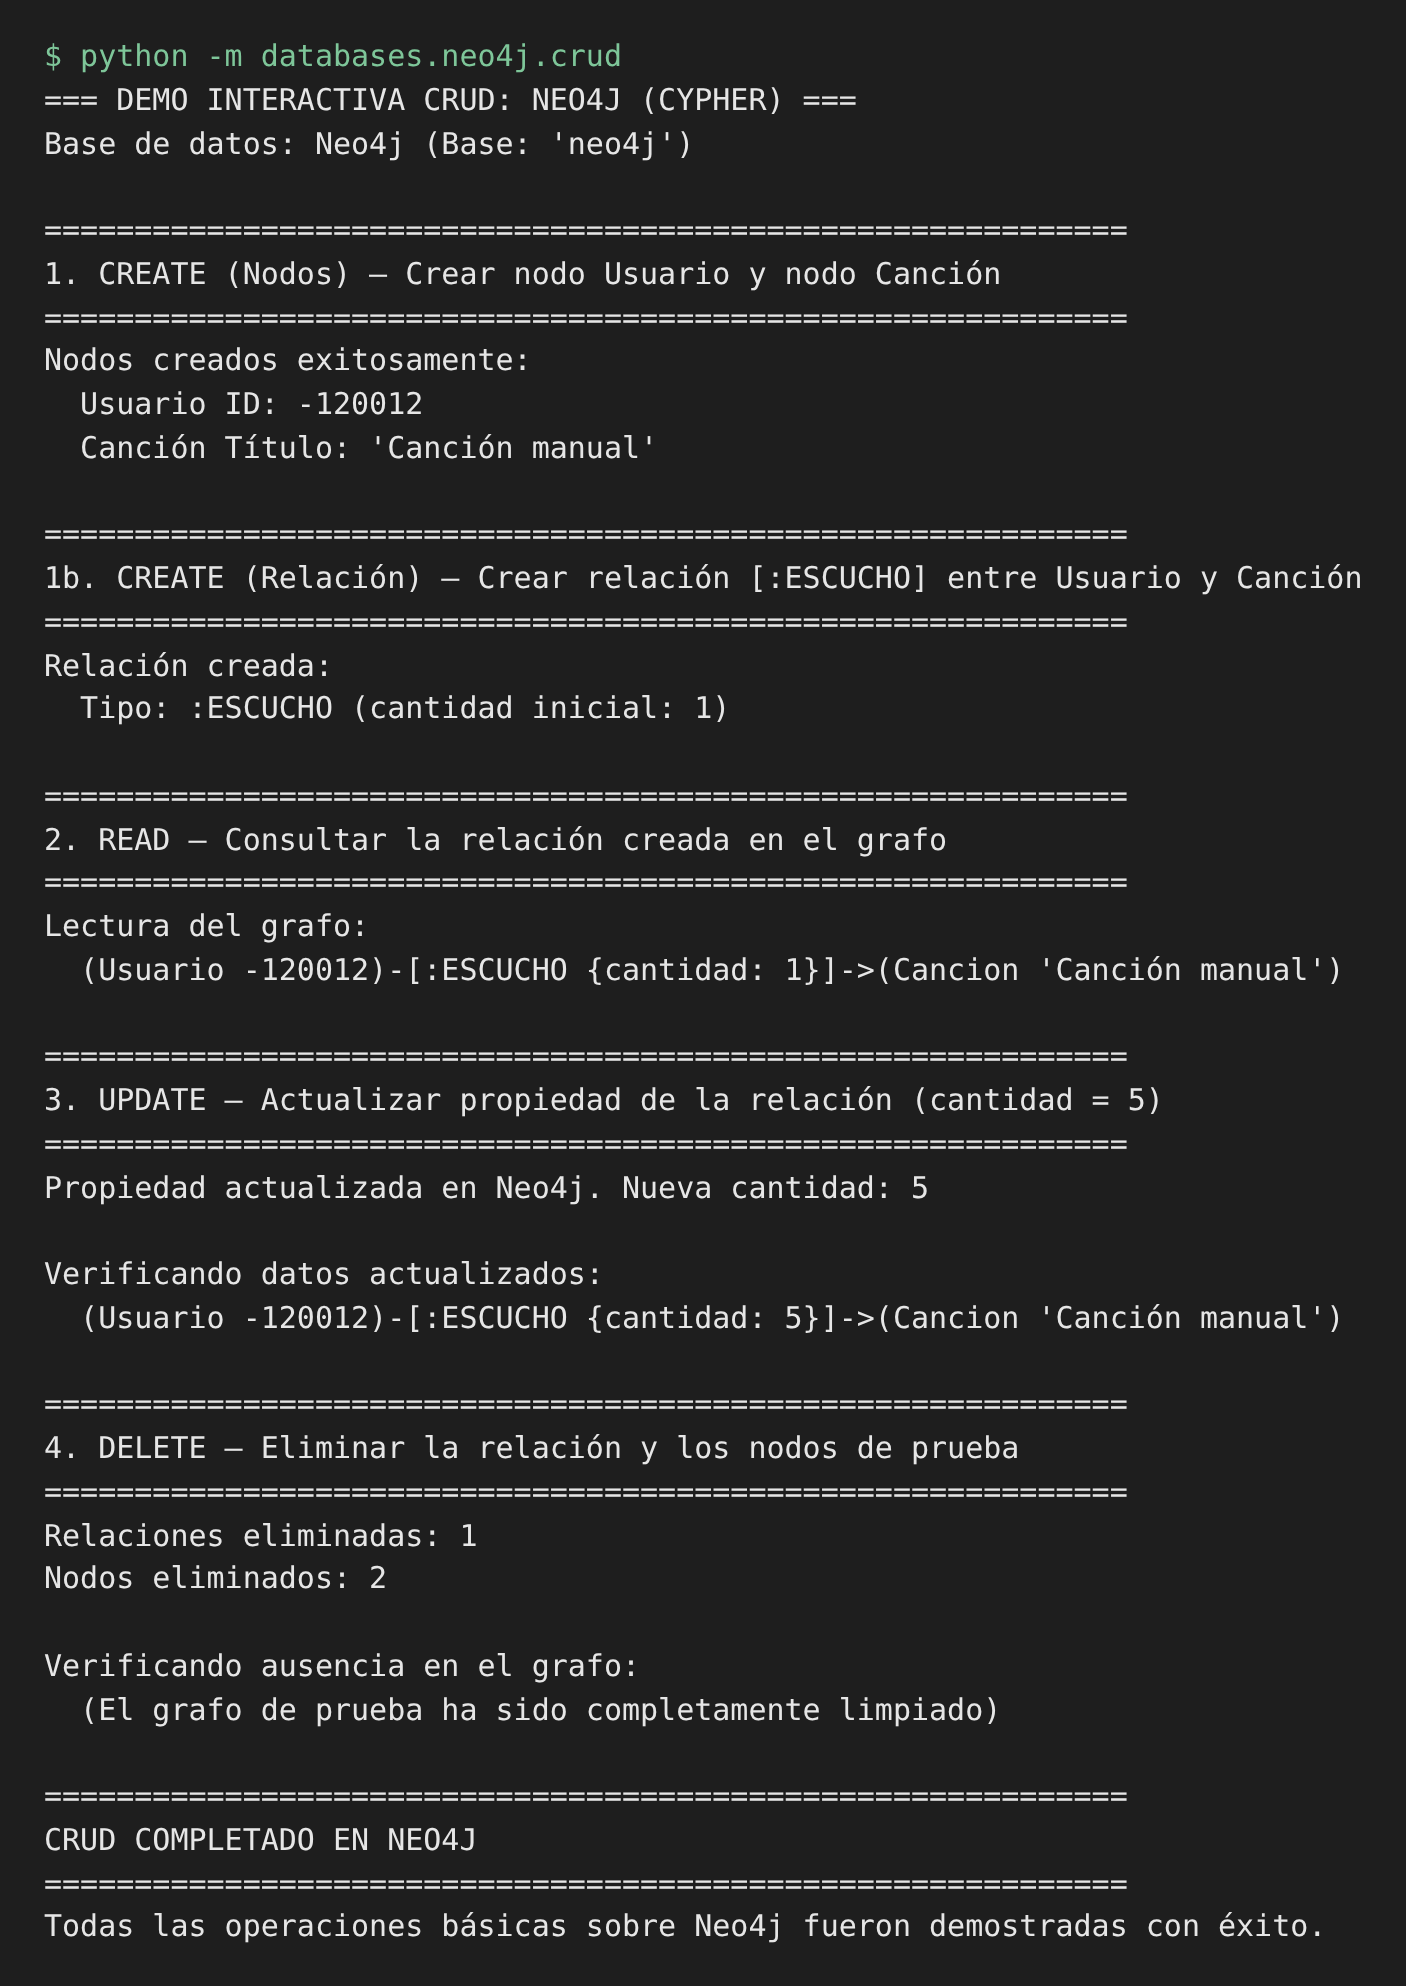
\includegraphics[width=0.68\textwidth]{figuras/neo4j_crud.png}
\end{figure}

\subsection{Afinidades y comunidades}

El análisis (\code{databases/neo4j/analyze.py}) usa los 500 artistas con más oyentes (al menos 20 cada uno). Para cada usuario se toman sus 20 artistas más escuchados y la audiencia $A(a)$ de un artista es el conjunto de usuarios que lo tienen en ese top. La afinidad entre dos artistas es el índice de Jaccard de sus audiencias:

\[
J(a,b) = \frac{|A(a) \cap A(b)|}{|A(a) \cup A(b)|}
\]

Se conservan los pares con al menos 10 usuarios en común y $J \geq 0{,}05$, y los 10 vecinos más afines de cada artista. Sobre ese grafo ponderado se detectan comunidades con Louvain (resolución 1, semilla 42) y se guardan en Neo4j las relaciones \code{AFIN_A}, las comunidades y los indicadores.

El coeficiente puente de cada artista mide cómo se reparten sus conexiones entre comunidades. Si $w_{a,c}$ es la suma de los pesos de Jaccard de las aristas de $a$ hacia artistas de la comunidad $c$ y $W_a$ la suma total:

\[
\text{puente}(a) = 1 - \sum_{c} \left( \frac{w_{a,c}}{W_a} \right)^2
\]

Vale 0 si todas sus conexiones están en una comunidad y crece al repartirse. La diversidad de un usuario es la entropía de Shannon normalizada de sus escuchas entre comunidades, con $p_{u,c}$ la fracción de sus escuchas clasificadas en la comunidad $c$ y $k_u$ el número de comunidades que escucha:

\[
D(u) = -\frac{\sum_{c} p_{u,c} \ln p_{u,c}}{\ln k_u}
\]

con $D(u) = 0$ si escucha una sola comunidad. Las tablas~\ref{tab:neo4j-analisis} y~\ref{tab:neo4j-comunidades} resumen el resultado.

\begin{table}[H]
\centering
\caption{Resultado del análisis de afinidades y comunidades}
\label{tab:neo4j-analisis}
\begin{tabular}{l r}
\toprule
Medida & Resultado \\
\midrule
Artistas seleccionados & 500 \\
Artistas conectados / aislados & 425 / 75 \\
Afinidades retenidas & 1\,553 \\
Comunidades & 13 \\
Modularidad ponderada & 0,782546 \\
Usuarios con recomendaciones & 16\,372 \\
Cobertura sobre los usuarios del lote & 62,03~\% \\
Escuchas clasificadas en comunidades & 1\,153\,631 (23,76~\%) \\
Diversidad media de usuarios clasificados & 0,416633 \\
\bottomrule
\end{tabular}
\end{table}

\begin{table}[H]
\centering
\caption{Comunidades detectadas}
\label{tab:neo4j-comunidades}
\begin{tabular}{r r r l}
\toprule
Comunidad & Artistas & Audiencia & Primeros representantes \\
\midrule
1 & 39 & 3\,556 & Travis Scott, Kendrick Lamar, Future \\
2 & 86 & 6\,585 & Linkin Park, Three Days Grace, Korn \\
3 & 84 & 6\,348 & Ariana Grande, Charli xcx, Taylor Swift \\
4 & 85 & 5\,545 & The Rolling Stones, Metallica, AC/DC \\
5 & 15 & 1\,611 & Ado, YOASOBI, Eve \\
6 & 17 & 1\,217 & Jin, Jimin, j-hope \\
7 & 11 & 1\,219 & Moby, Massive Attack, Air \\
8 & 13 & 1\,131 & ILLIT, LE SSERAFIM, aespa \\
9 & 65 & 6\,310 & Malcolm Todd, The Smiths, Radiohead \\
10 & 2 & 209 & Bill Withers, Marvin Gaye \\
11 & 2 & 246 & Crystal Castles, Grimes \\
12 & 2 & 242 & Hans Zimmer, Max Richter \\
13 & 4 & 533 & Royal Blood, The Black Keys, Nothing But Thieves \\
\bottomrule
\end{tabular}
\end{table}

Las comunidades agrupan artistas cercanos (rap estadounidense, metal y rock alternativo, pop, rock clásico, J-pop, solistas de BTS, música electrónica, K-pop); sus números identifican una partición concreta. Los representantes son los artistas con mayor grado ponderado de cada comunidad.

\subsection{Recomendaciones y consultas}

La recomendación para un usuario suma, por cada artista que aún no escucha, su afinidad con los artistas que sí escucha, ponderada por el peso de cada uno en su historial:

\[
\text{puntaje}(u, n) = \sum_{k \in K(u)} \text{proporcion}(u,k) \cdot J(k,n)
\]

donde $K(u)$ son los artistas que escucha $u$. La consulta devuelve también la evidencia (artista conocido y Jaccard):

\begin{lstlisting}[language=Cypher]
MATCH (l:Lote {id:$dataset, estado:'completo'})-[:ANALISIS_ACTIVO]->(an:Analisis)
MATCH (u:Usuario {id:$user})-[p:ESCUCHA_ARTISTA {lote:l.id}]->(conocido:Artista)
MATCH (conocido)-[f:AFIN_A {analisis:an.id}]-(nuevo:Artista)
WHERE NOT EXISTS { MATCH (u)-[:ESCUCHA_ARTISTA {lote:l.id}]->(nuevo) }
WITH nuevo, sum(p.proporcion * f.jaccard) AS puntaje,
     collect({artista_conocido:conocido.nombre, jaccard:f.jaccard}) AS evidencia
RETURN nuevo.nombre AS artista, puntaje, evidencia
ORDER BY puntaje DESC LIMIT $limit
\end{lstlisting}

Por ejemplo, una escucha de Motörhead lleva a recomendar Judas Priest: comparten 17 oyentes, con Jaccard 0,091892 y puntaje 0,032819. La consulta de canciones devuelve \emph{Breaking the Law}, y el camino más corto entre ambos artistas tiene un salto. Radiohead aparece con coeficiente puente 0,634146.

\code{python -m databases.neo4j.queries} ejecuta el resto de consultas: artistas con más oyentes, canciones de un artista, escuchas de un usuario, búsqueda por texto, totales del lote, recomendación de canciones, comunidades, artistas puente, diversidad e indicadores del análisis. La de artistas con más oyentes la usa Airflow para el KPI 5 (sección~\ref{cap:kpis}).
